\chapter{Approach}
\label{cha:approach}

The purpose of this thesis is to perform an empirical comparison of forecasting methods. In order to do this, suitable methods, assets and systems need to be identified and evaluated.
This chapter identifies the requirements these need to fulfill in order to be suitable for use in a benchmarking system. Further this chapter identifies assets and methods which need to be investigated further in a small experimental study to determine their suitability. In chapter \ref{cha:designing} the results of this small experimental study is presented. The concepts discussed in this chapter are then combined into a benchmarking toolkit for forecasting methods which is presented in chapter \ref{cha:crayon}. This system is then used for the empirical comparison in chapter \ref{cha:chapter6}.

\section{Defining reproducibility}
In section \ref{sec:reproducibility} the term reproducibility was split into three categories; \textit{technical}, \textit{statistical} and \textit{conceptual}. A benchmarking toolkit should adhere to the requirements posed by these rules in order to be reproducible, thus following requirements need to be met:

In addition to these points, automating the benchmark would lead to a higher degree of reproducibility as the benchmarks would be standardized and thus less error prone. However, certain aspects of a benchmark, such as the error metric, are not suitable to be standardized since which error metric should be used depends on the use case.

\begin{figure}[h]
  \begin{enumerate}
    \item Encapsulation tools should be used for dependency and algorithm management.
    \item Experiments should run multiple times in order to build up a distribution of errors such that the variance of the error is recorded.
    \item Statistical tests should be applied to the results to enforce statistical reproducibility.
    \item Multiple datasets should be used when benchmarking to cover various usecases for conceptual reproducibility.
  \end{enumerate}
  \caption{Requirements for a reproducible benchmark.}
  \label{fig:reproducibility_requirements}
\end{figure}

\section{Defining fair comparisons}
\label{sec:fair_comparisons}
The adjective Fair is defined as \textit{acceptable and appropriate in a particular situation.} in the Oxford Dictionary. When benchmarking forecasting models, one method of achieving fair comparisons is to evaluate algorithms on multiple complementary datasets as this showcases the strengths and weaknesses of algorithms in different scenarios. Additionally, fair comparisons also require that the variance is shown as this provides more detail of an algorithms overall performance than a single value \cite{bouthillier2021accounting}.

Simply executing an algorithm on multiple datasets is not enough as it is important to give each algorithm a fair opportunity to perform well on each dataset. This is normally achieved by \textit{tuning} the hyperparameters of an algorithm for the dataset in question. A fair way of tuning algorithms is however non trivial as different strategies tend to be biased \cite{sivaprasad2020optimizer}. One method of achieving fairness could be to limit the time spent for hyperparameter tuning to some constant value. This would however be unfair towards slower methods such as DNNs or RNNs as the search space traversed would be smaller when compared to faster models such as simple NNs or classical models. Another approach is to limit the size of the search space by limiting the number of hyperparameter configurations to be tested. This would benefit models with few hyperparameters as each hyperparameter would be more thoroughly tuned than if more hyperparameters would be available. The inverse of this would also hold, one could limit the number of configurations for each hyperparameter tested but let the total number of hyperparameter configurations to be unbound. This would however be unfair towards models with few parameters.

Another approach would be to tune each algorithm such that it achieves its \textit{optimal} performance for each dataset. This would be fair in the sense that it is independent of the complexity of the algorithm being tested. For ML competitions this is commonly the case as contestants tune their algorithms to perform optimally in order to win \cite{roelofs2019meta}. This is also the case when algorithms are used in practice as companies and organizations leveraging machine learning, spend considerable effort in tuning these to fit their data \cite{beam2020challenges}.

To enable fair comparisons the implementations of the models being compared should be bug free and optimized. This is especially important for very complex models as the engineering effort of implementing such algorithms correctly is considerable.

A summary of the requirements for fair comparisons which have been identified is presented in \ref{fig:fair_requirements}
\begin{figure}[h]
  \begin{enumerate}
    \item Optimally tuned algorithms for each dataset
    \item Variance should be reported
    \item Models should be evaluated on multiple complementary datasets
    \item Reference implementations of tested forecasting models should be used when possible
  \end{enumerate}
  \caption{Requirements for a fair benchmark.}
  \label{fig:fair_requirements}
\end{figure}

\section{Defining accurate comparisons}
In section \ref{subsec:error_metrics} different metrics were presented for comparing forecasting accuracy. It was established that error metrics have different strengths and weaknesses which makes different metrics suitable for different domains or applications.
Thus, in order to perform an accurate comparison of forecasting methods via a benchmarking system, multiple different metrics need to be made available.

\begin{figure}[htb]
  \centering
  \minipage{0.47\textwidth}
  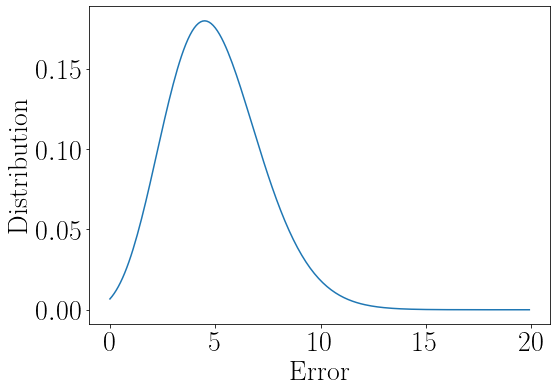
\includegraphics[width=\linewidth]{./img/poisson_distribution.png}
  \caption{Poisson distribution}
  \label{fig:poisson_distribution}
  \endminipage\hfill
  \minipage{0.47\textwidth}
  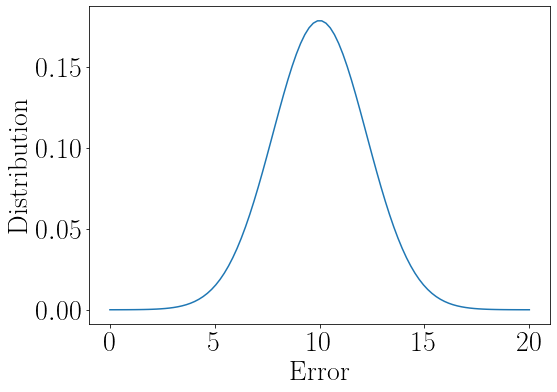
\includegraphics[width=\linewidth]{./img/normal_distribution.png}
  \caption{Gaussian distribution}
  \label{fig:normal_distribution}
  \endminipage\hfill
  \caption{Which error distribution is better?}
  \label{fig:example_distributions}
\end{figure}


Since, for reproducibility purposes, each model shall generate a distribution of error metrics one cannot any longer compare algorithms based on single metric values. In figure \ref{fig:example_distributions} two examples of possible error distributions are presented. Since a smaller error is generally considered better, it makes sense that distributions which are concentrated around zero perform the best. For example in Figure \ref{fig:example_distributions} an algorithm generating an error distribution such as the poisson is more likely to produce errors close to 0 than an algorithm with an error distribution like the normal distribution in Figure \ref{fig:normal_distribution}.

A summary of what is required to perform accurate comparisons is presented in \ref{fig:accurate_requirements}.

\begin{figure}[h]
  \begin{enumerate}
    \item Suitable error metrics should be used for the domain and datasets.
    \item The distribution of the error metric over multiple runs is used when comparing different algorithms.
  \end{enumerate}
  \caption{Requirements for accurate comparisons}
  \label{fig:accurate_requirements}
\end{figure}

% \section{Ensuring reproducible results}
% \label{"sec:reproducibility"}
% The ability to reproduce findings is a core tenet of the scientific method. Deep learning often has some randomness associated to it which makes reproducing results more difficult. In \ref{subsec:defining_reproducibility} we define reproducibility for deep learning. Section \ref{subsec:distributions} dives deeper into how distributions of error metrics can be used to ensure reproducibility of experiments.

% \subsection{Defining reproducibility}
% \label{subsec:defining_reproducibility}
% As discussed in \ref{subsec:reproducibility} deep learning models often suffer from random fluctuations in their accuracy due to inherent random processes of their architectures. This makes it hard to accurately and reproducibly compare the accuracy of different algorithms.

% A common approach to solve this randomness is to fix the random seed prior to training the algorithm. While this does ensure that a specific configuration of the model is reproducible it does not necessarily ensure that the behaviour of an algorithm in general is reproducible.

% By not fixing the seed we will instead receive a distribution of errors for a given hyperparameter configuration. This distribution provides insights into what range of accuracies one could expect for a specific algorithm running on a specific dataset. I.e. is it heavy tailed, is it wide, does it follow a normal distribution etc. By instead comparing distributions of algorithm errors we can more generally verify if two algorithms perform the same. Thus by our definitions, if two algorithms perform the same they are, logically equivalent in performance.

% It is somewhat common that code needed for running algorithms are provided by by their authors. However, it is unfortunately not always the case that the code is frozen at the time of publication. I.e. additional changes may have been added to the algorithm since its publication. This complicates matters as different implementations of the same algorithm may behave differently (gluonts bug on deepar). Furthermore, different implementations of the same algorithm may have different parameters exposed/different internal architecture thus possibly resulting in different results on the same workload (SageMaker DeepAR vs GluonT DeepAR).

% Due to this I believe that persistent artifacts such as Docker images containing algorithms are needed for true reproducibility. In \ref{subsec:runtool} I present a purpose built tool which through a domain specific language allows defining experiments on algorithms in Docker images. By sharing the docker image, a configuration file, the dataset and a small python script reproducible runs of an algorithm can be made.

% To summarize, in this thesis, reproducibility is defined as being able to verify whether two independent sets of training jobs are sampled from the same distribution. Furthermore, for strong reproducibility I propose that algorithm artifacts such as Docker images are used in conjunction with a reproducible way of running them.

% \subsection{A look on distributions}
% \label{subsec:distributions}
% Suppose that I would publish a report detailing that on error metric X on dataset D it receives a value of E. This approach is analogous to saying that "this method with these specific parameters outputs this value". By limiting the representation of the algorithm to this extent one is unable to capture additional characteristics of the algorithm such as how consistent its errors are.

% Some randomness cannot be controlled by setting the seed such as OS related scheduling of threads. This can effect the performance of ML models using multi-threading for fast calculations (SEE SECTION XYZ FOR MORE). If this kind of error occurs, it may be hard to reproduce results.

% TODO look through the paragraphs below and bind them together better.

% Running an algorithm on a dataset N  times would result in a set of N error metrics being produced. These errors would be samples taken from a distribution of the errors this specific algorithm would have on this specific dataset. One could imagine that an algorithm which generally performs well on this dataset would have an error distribution with a peak close to the metrics optimum value (i.e. 0 for MASE, MAPE, AE etc.). Furthermore, algorithms with a higher variance in their results, should logically result in a wider distribution.

% In the following sections I will discuss possible approaches to solve the following questions:

% \begin{enumerate}
%     \item How can one verify that two sets of error metrics; N and M are sampled using the same forecasting algorithm on a specific dataset.
%     \item How accurate is the method in terms of false positives.
%     \item What sample size does it need to work sufficiently well. TODO define sufficiently well...
%     \item How does it perform empirically
% \end{enumerate}

% \section{Enabling fair and accurate comparisons}
% \label{sec:fair_and_accurate_comparisons}
% \subsection{Equal tuning effort}
% \label{subsec:equal_tuning}
% When machine learning algorithms are employed in real life these algorithms are tuned thoroughly on the data it should predict on.

% In order to allow for fair comparisons between models, it is required that the algorithms has been tuned on the dataset in question. Performing tuning in a fair way is hard as there are many strategies one could employ to ensure a fair tuning effort. However none of these strategies are flawless and thus, some algorithms may be better tuned using one strategy than another.

% One strategy which could be employed to ensure fair tuning could be to fix the total training time available for tuning. This would be fair in the sense that each algorithm would have the same time to find good hyperparameters. However this would give an unfair advantage to fast algorithms. Further, even the programming language used to develop a system could bias these results. I.e. the programming language C generally executes faster than for example Python.

% Another strategy could be to set a fixed amount of parameter combinations to test. This ensures that the search space of the parameters are equally traversed for different algorithms. However it is not fair in the sense that the search space of some algorithms hyperparameter configurations are larger than others. Thus an algorithm with two hyperparameters would be more comprehensively tuned than an algorithm with hundreds of parameters.

% \subsubsection{User tuned}
% \subsubsection{Automated tuning}

% \subsection{Metrics}

% \section{Designing a benchmarking system for forecasting methods}

% \subsection{Choosing datasets}
% \subsection{Handling reproducibility}
% \subsubsection{Naive approach}
% Random noise follows a normal distribution if enough samples are taken. Thus if the noise added to the errors is purely random noise, it follows that the distributions of the error metrics should be normally distributed. TODO verify/come with examples

% If this is the case, then one should be able to detect if N is sampled from the same distribution as M by comparing the mean of N with the mean of M +- some standard deviations of M. This approach has the benefit of being simple and intuitive.
